% DSA4212 - Optimisation for Large-Scale Data-Driven Inference
% Small-LLM challenge report. Course Overleaf template (12pt, natbib, libertine).
% Figures are in report/figures/; bibliography in report/references.bib.
\documentclass[12pt]{article}

%%%%%%%%%%%%%%%%%%%%%%%%%%%%%%%%%%%%%%%%%%%%%%%%%%%%%%%%%%%%%%%%%%%%%%%%%%%%%%%%%%%%%%
%%%%%%%%%%%%%%%%%%% YOU PROBABLY DON"T NEED TO CHANGE ANYTHING HERE %%%%%%%%%%%%%%%%%%%
\usepackage[numbers,sort]{natbib}
\usepackage{amsfonts, amsmath}
\usepackage{graphicx}
\usepackage{booktabs}   % for the results tables (\toprule etc.)
\IfFileExists{libertine.sty}{\usepackage{libertine}}{} % template font (present on Overleaf)
\usepackage{fullpage}
\usepackage{hyperref}
\hypersetup{
    colorlinks = true,
    linkcolor = blue,
    urlcolor  = blue,
    citecolor = blue,
    anchorcolor = blue}
\urlstyle{same}
\IfFileExists{microtype.sty}{\usepackage{microtype}}{} % tighter line breaking
\setlength{\emergencystretch}{3em} % avoid lines running into the margin
\Urlmuskip=0mu plus 1mu\relax      % let URLs flex so they do not overrun
%%%%%%%%%%%%%%%%%%%%%%%%%%%%%%%%%%%%%%%%%%%%%%%%%%%%%%%%%%%%%%%%%%%%%%%%%%%%%%%%%%%%%%

\title{Training a small GPT on TinyStories under a one-hour budget:
a compute-optimal sweet spot}
\date{\today}

\begin{document}

\maketitle

{\bf Group Composition:}
\begin{enumerate}
\item Lara Muy Steffany Mishell (Steffany Lara), A0350565H, [NUS email]
\item Kerem Ozemre, A0[fill], [NUS email]
\item Kowalke Jeri Tonio Janek (Tonio Kowalke), A0[fill], [NUS email]
\item Haj Hassine Ahmed Ben Abdellaziz (Ahmed Haj Hassine), A0[fill], [NUS email]
\end{enumerate}

{\bf Github Repository:}
\href{https://github.com/KeremOzemre/Optimization-for-Large-Scale-Data}{github.com/KeremOzemre/\allowbreak Optimization-for-Large-Scale-Data}

\begin{abstract}
We trained 20 nanoGPT language models on TinyStories from random weights, each for
one hour on the same GPU: five model sizes (16 to 253M parameters) crossed with four
training-data fractions (25/50/75/100\% of the training split). The tokenizer,
optimizer, schedule, context length, and effective batch were held fixed, so the
only things that changed were model size and how much data each run could draw from.
Validation loss drops steeply from \texttt{small} to \texttt{xl} ($\approx$124M
parameters) and then gets slightly worse again at \texttt{xxl} ($\approx$253M). The
reason is simple once you look at throughput: \texttt{xxl} is so slow that it only
gets through about half as many tokens in the hour, so it stays undertrained. The
data fraction barely moves the loss, because no run gets through even 25\% of the
split in the time it has. Picking the best model by validation loss gives
\texttt{xl\_data50} (val loss 1.5025, perplexity 4.49); on the untouched test split
it reaches loss 1.4846, perplexity 4.41, and 0.524 bits per byte.
\end{abstract}

\section{Compute budget declaration}
Every model starts from random weights (nanoGPT initialisation, with no pretrained
weights, embeddings, or tokenizer fine-tuning) and trains for exactly one hour
(3600\,s) of in-loop wall-clock per model. Data preparation, the final validation
pass, and checkpointing all happen outside that timed loop. All 20 runs use the same
hardware: a single NVIDIA H100 NVL MIG 3g.47gb slice in \texttt{bfloat16}. The same
hour of wall-clock does not buy the same number of tokens for every size, and that
gap turns out to drive our main result (\S\ref{sec:results}).

\section{Research question}
Which model size and training-data fraction give the best language-modeling
performance under a fixed one-hour budget on identical hardware? We hold the
tokenizer, optimizer, schedule, context length, and effective batch size fixed, and
vary only (a) model size and (b) the fraction of the training split used.

\section{Experimental setup}
\begin{itemize}
  \item \textbf{Data:} \texttt{roneneldan/TinyStories}. We train on the official
        train split, and split the official validation set 80/20 into validation and
        test at the story level (seed 42). The test split is only touched once, for
        the final comparison (\S\ref{sec:test}).
  \item \textbf{Tokenizer:} GPT-2 (\texttt{tiktoken}), vocabulary 50{,}257, with an
        end-of-text token after every story. Since the tokenizer never changes,
        per-token cross-entropy and perplexity are directly comparable across all our
        runs.
  \item \textbf{Model:} nanoGPT~\cite{karpathy} GPT with tied input/output
        embeddings, causal self-attention, context length 256, and dropout 0.1.
  \item \textbf{Evaluation objective:} held-out cross-entropy on the test split,
        also reported as perplexity ($\exp$ of the loss) and bits per byte.
        Cross-entropy is the quantity the model is trained on, measured on unseen
        text, so it reads language-modeling quality directly; perplexity is its
        interpretable version; and bits per byte lets our numbers be compared to work
        that uses a different tokenizer~\cite{eldan2023}. Splitting at the story level
        with seed 42 keeps any single story from leaking between validation and test.
\end{itemize}

\begin{table}[h]
  \centering
  \caption{The five model sizes. Width divides evenly by the head count; context
  length (256) and dropout (0.1) are shared. We adjust microbatch and accumulation to
  keep an effective batch of 16 sequences (4096 tokens) per optimizer step at every
  size.}
  \label{tab:sizes}
  \begin{tabular}{lrrrrr}
    \toprule
    Size & Layers & Width & Heads & Params (M) & Microbatch $\times$ accum. \\
    \midrule
    \texttt{small}  &  4 &  256 &  4 &  16.08 & $16 \times 1$ \\
    \texttt{medium} &  6 &  384 &  6 &  30.02 & $16 \times 1$ \\
    \texttt{large}  &  8 &  512 &  8 &  51.04 & $16 \times 1$ \\
    \texttt{xl}     & 12 &  768 & 12 & 123.75 & $\phantom{0}8 \times 2$ \\
    \texttt{xxl}    & 16 & 1024 & 16 & 253.09 & $\phantom{0}4 \times 4$ \\
    \bottomrule
  \end{tabular}
\end{table}

\noindent\textbf{Data fractions:} 25/50/75/100\% of the training split, giving a
$5\times4$ grid of 20 runs. \textbf{Optimizer and schedule:} AdamW (lr
$3\times10^{-4}$, weight decay 0.1, betas 0.9/0.95, gradient clip 1.0), with a
time-based 2\% warmup and then cosine decay to 10\% of the peak learning rate.

\section{Methodology and reproducibility}
The exact commands are in the repository README; the pipeline is five steps.
\begin{enumerate}
  \item \texttt{run.py prepare} builds (or reuses) the token cache for a given data
        fraction.
  \item \texttt{create\_experiments.py} writes the per-run configs under
        \texttt{configs/experiments/} from the baseline YAML.
  \item \texttt{run.py train} trains one config; its outputs
        (\texttt{run\_config.json}, \texttt{metrics.csv}, \texttt{checkpoint.pt}) land
        in \texttt{results/}. Checkpoints and logs are mirrored to the Hugging Face
        Hub (\texttt{dsa4212-tinystories}).
  \item We pick the model on \emph{validation} loss, and only then score the chosen
        one on \emph{test}.
  \item \texttt{eval\_hf.py} downloads every checkpoint and scores the full test
        split; \texttt{analyze.py} then aggregates all runs into \texttt{analysis/}
        (the tables and figures below).
\end{enumerate}

\section{Results}\label{sec:results}
Table~\ref{tab:results} lists all 20 runs sorted by final validation loss, the metric
we select on. We read three things off these runs, shown in
Figures~\ref{fig:curves}--\ref{fig:tension}.

\begin{table}[h]
  \centering
  \caption{All 20 runs, sorted by final validation loss (the selection metric).
  ``Tokens'' is how many training tokens the run actually processed inside the
  one-hour budget. Test numbers are shown for completeness, but we did not use them to
  select the model (\S\ref{sec:test}).}
  \label{tab:results}
  \small
  \begin{tabular}{lrrrrrr}
    \toprule
    Run & Params (M) & Data\% & Tokens (M) & Val loss & Val ppl & Test ppl \\
    \midrule
    \texttt{xl\_data50}      & 123.75 &  50 & 273.9 & \textbf{1.5025} & \textbf{4.49} & 4.41 \\
    \texttt{xl\_data100}     & 123.75 & 100 & 279.8 & 1.5068 & 4.51 & 4.40 \\
    \texttt{xl\_data75}      & 123.75 &  75 & 269.1 & 1.5099 & 4.53 & 4.43 \\
    \texttt{xxl\_data100}    & 253.09 & 100 & 143.7 & 1.5106 & 4.53 & 4.56 \\
    \texttt{xl\_data25}      & 123.75 &  25 & 283.3 & 1.5118 & 4.54 & 4.45 \\
    \texttt{xxl\_data75}     & 253.09 &  75 & 141.1 & 1.5125 & 4.54 & 4.59 \\
    \texttt{xxl\_data50}     & 253.09 &  50 & 148.2 & 1.5155 & 4.55 & 4.56 \\
    \texttt{xxl\_data25}     & 253.09 &  25 & 143.2 & 1.5233 & 4.59 & 4.61 \\
    \texttt{large\_data100}  &  51.04 & 100 & 562.4 & 1.5460 & 4.69 & 4.66 \\
    \texttt{large\_data75}   &  51.04 &  75 & 562.0 & 1.5466 & 4.70 & 4.67 \\
    \texttt{large\_data50}   &  51.04 &  50 & 557.9 & 1.5479 & 4.70 & 4.69 \\
    \texttt{large\_data25}   &  51.04 &  25 & 563.2 & 1.5509 & 4.72 & 4.70 \\
    \texttt{medium\_data100} &  30.02 & 100 & 734.6 & 1.6444 & 5.18 & 5.16 \\
    \texttt{medium\_data75}  &  30.02 &  75 & 738.3 & 1.6462 & 5.19 & 5.17 \\
    \texttt{medium\_data50}  &  30.02 &  50 & 737.3 & 1.6527 & 5.22 & 5.20 \\
    \texttt{medium\_data25}  &  30.02 &  25 & 719.1 & 1.6558 & 5.24 & 5.21 \\
    \texttt{small\_data75}   &  16.08 &  75 & 940.8 & 1.8383 & 6.29 & 6.28 \\
    \texttt{small\_data100}  &  16.08 & 100 & 984.3 & 1.8386 & 6.29 & 6.26 \\
    \texttt{small\_data50}   &  16.08 &  50 & 985.5 & 1.8421 & 6.31 & 6.29 \\
    \texttt{small\_data25}   &  16.08 &  25 & 972.0 & 1.8452 & 6.33 & 6.31 \\
    \bottomrule
  \end{tabular}
\end{table}

\begin{figure}[h]
  \centering
  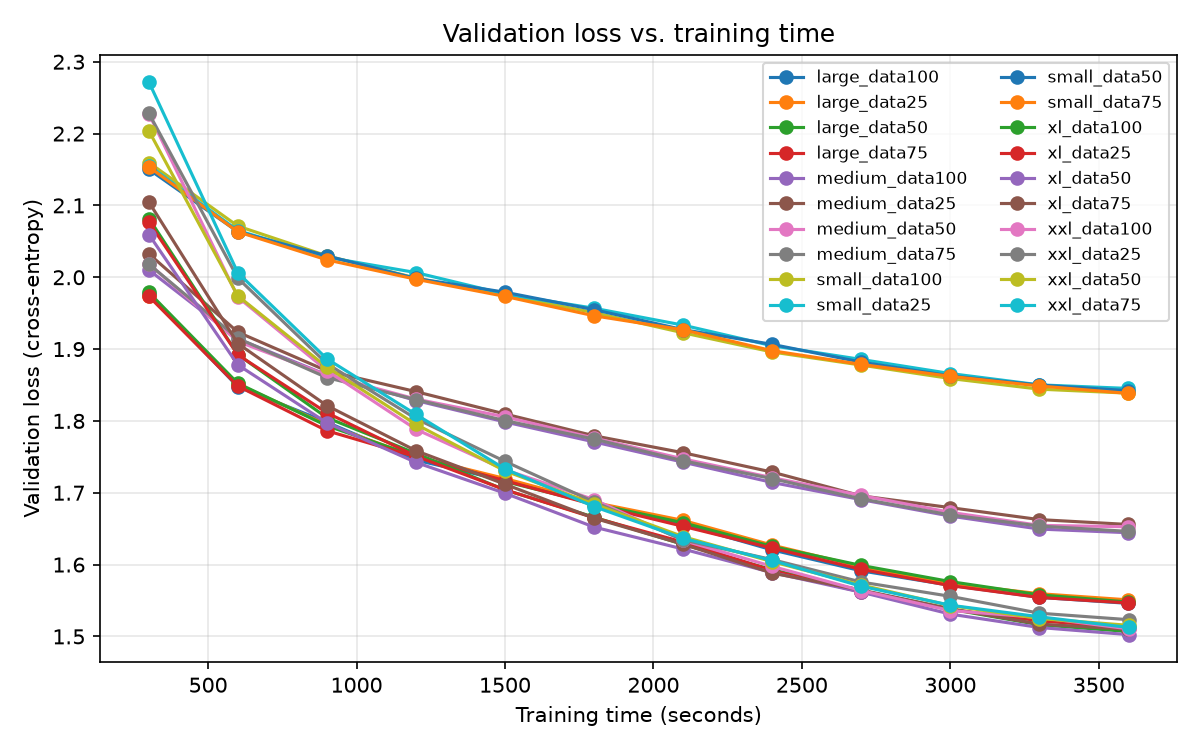
\includegraphics[width=0.75\linewidth]{figures/val_loss_curves.png}
  \caption{Validation loss over training time. The smaller models drop fastest early
  on, since they fit many more steps per second, and then flatten. \texttt{xl} and
  \texttt{xxl} start higher but pass the smaller models and are still coming down at
  the one-hour mark, which says they are limited by compute rather than converged.}
  \label{fig:curves}
\end{figure}

\begin{figure}[h]
  \centering
  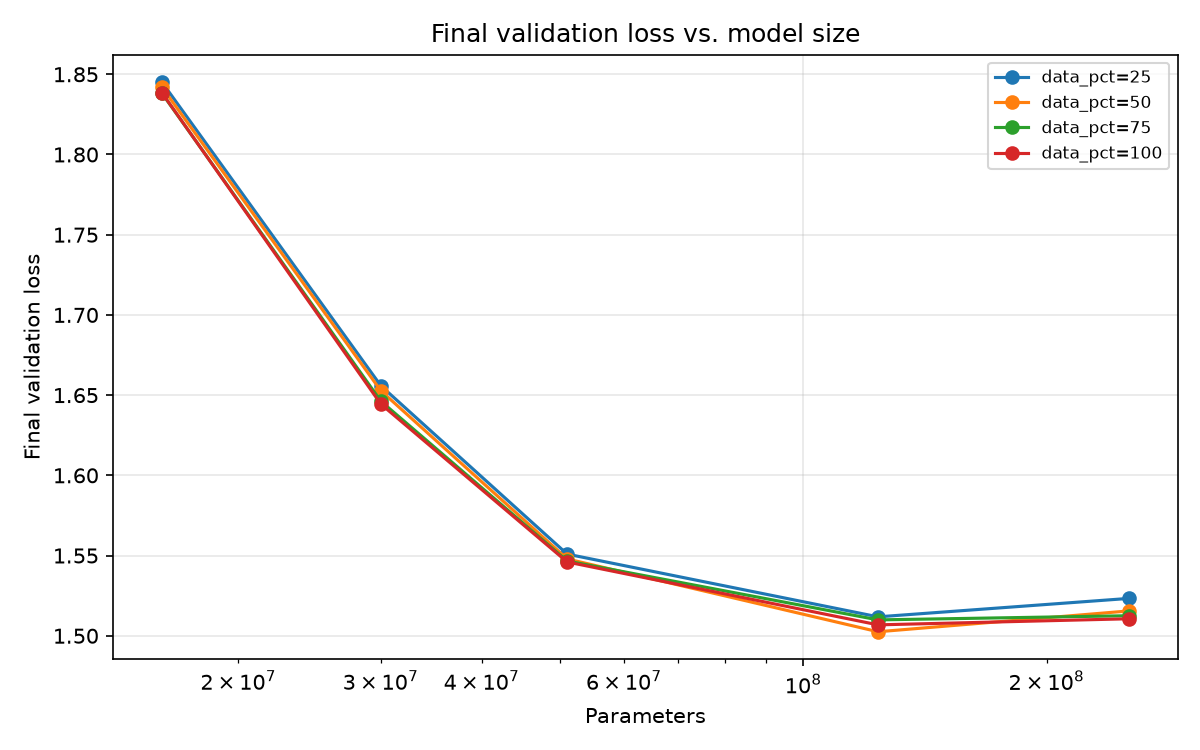
\includegraphics[width=0.49\linewidth]{figures/val_loss_vs_params.png}
  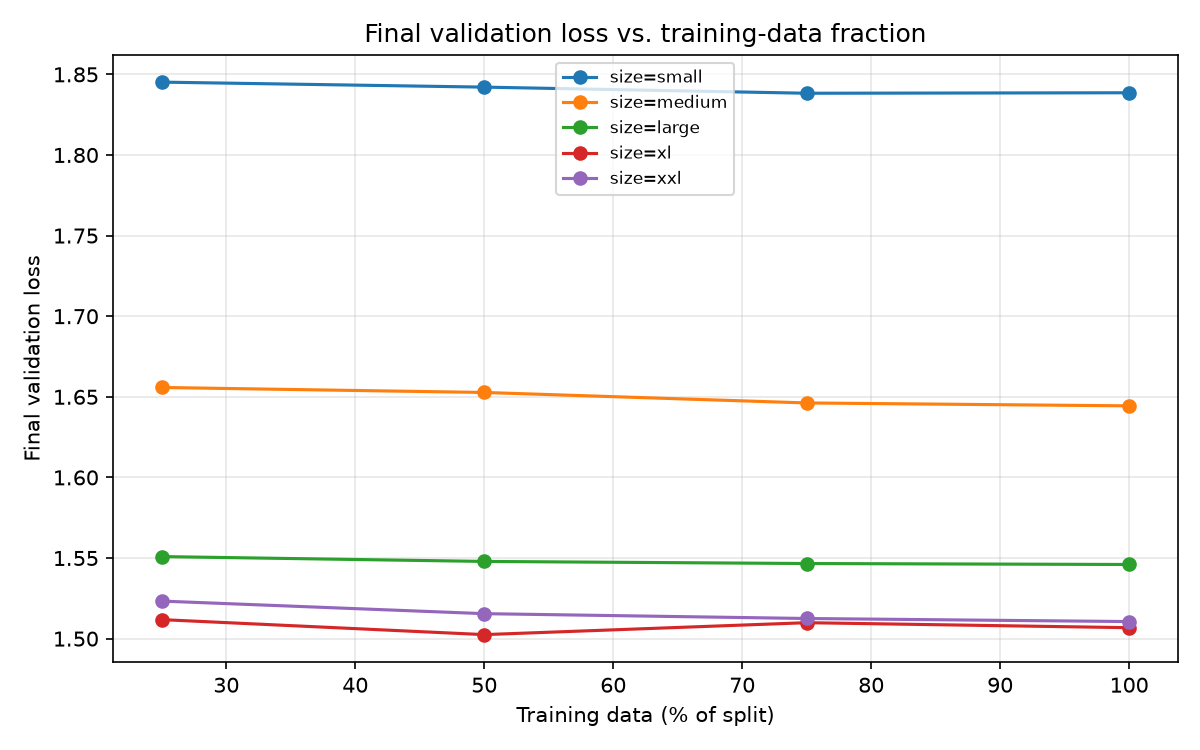
\includegraphics[width=0.49\linewidth]{figures/val_loss_vs_data.png}
  \caption{Left: final validation loss against model size, one line per data fraction.
  Loss falls steeply from \texttt{small} through \texttt{xl}, then ticks back up at
  \texttt{xxl}, leaving a sweet spot near 124M parameters. Right: loss against data
  fraction, one line per size. The lines are almost flat; within each size the four
  fractions differ by about 0.01 nats, and not even in a consistent direction.}
  \label{fig:sizedata}
\end{figure}

\begin{figure}[h]
  \centering
  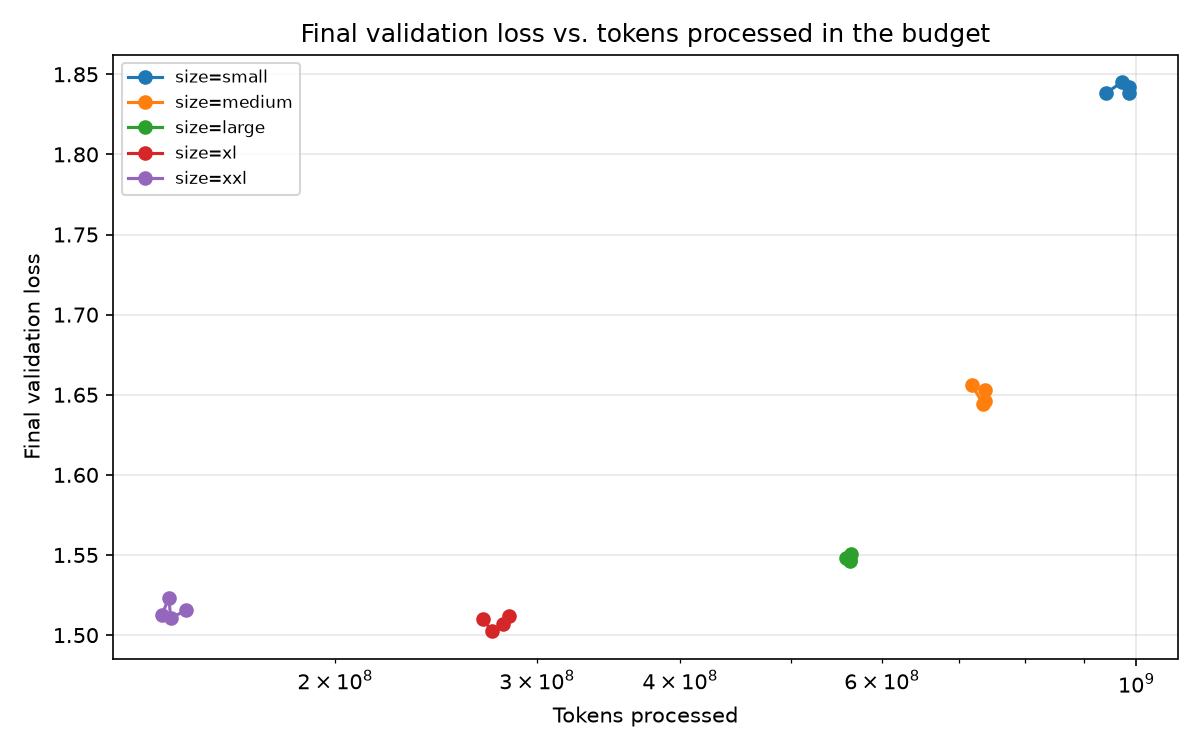
\includegraphics[width=0.49\linewidth]{figures/val_loss_vs_tokens.png}
  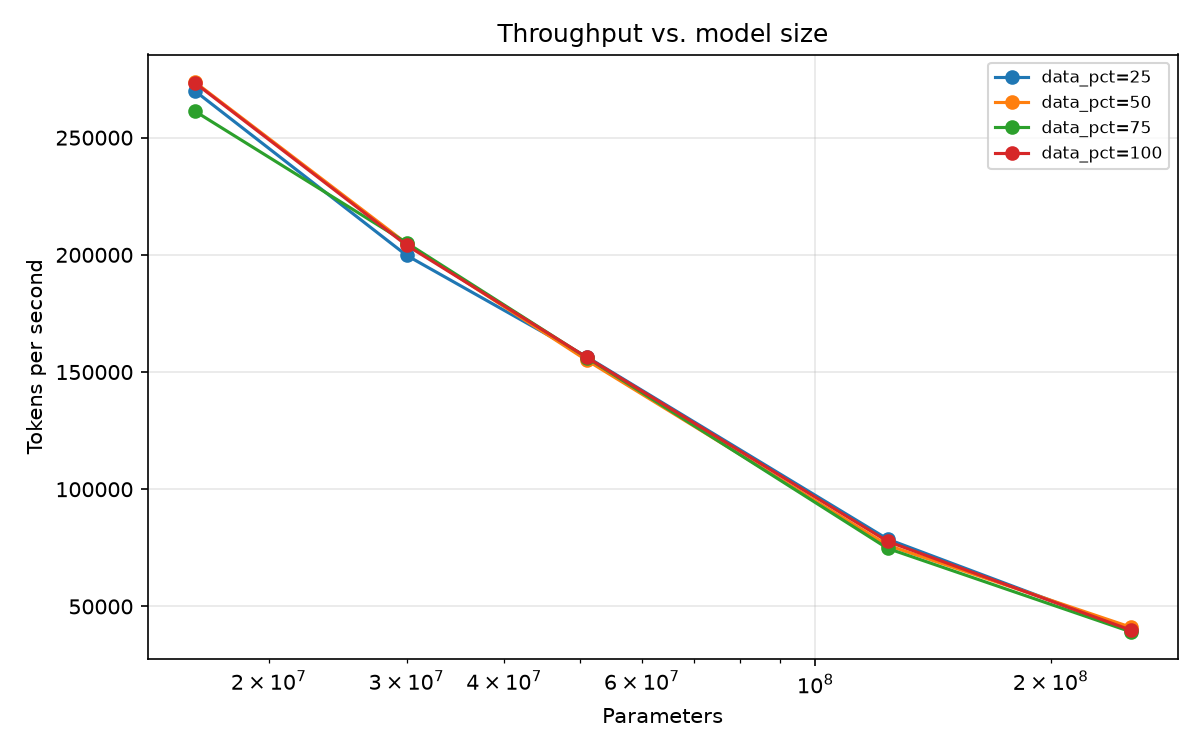
\includegraphics[width=0.49\linewidth]{figures/throughput_vs_params.png}
  \caption{Throughput against tokens seen in the hour. Right: throughput collapses as
  the model grows, from about 270k tokens/s for \texttt{small} down to about 40k for
  \texttt{xxl}. Left: so the larger models get through far fewer tokens in the same
  hour (about 985M for \texttt{small} versus 144M for \texttt{xxl}, roughly 7 times
  fewer), yet still reach lower loss per token, right up until \texttt{xxl}, where too
  few tokens finally cost more than the extra capacity is worth.}
  \label{fig:tension}
\end{figure}

\paragraph{(1) A compute-optimal sweet spot.} Bigger helps, with sharply diminishing
returns, and then stops helping. Validation loss falls $1.84\to1.64\to1.55\to1.50$
from \texttt{small} to \texttt{xl}, but the best \texttt{xxl} run (1.5106) comes out
above the best \texttt{xl} run (1.5025). \texttt{xxl} has about twice the parameters
of \texttt{xl} and runs at roughly half the throughput, so it only sees about 144M
tokens in the hour against 274M for \texttt{xl}, and never finishes training
(Fig.~\ref{fig:tension}). This is the compute-optimal picture of Hoffmann et
al.~\cite{hoffmann2022}: for a fixed compute budget there is a best model size, and
going past it spends the budget on parameters that never see enough tokens.

\paragraph{(2) The data fraction barely matters.} Within each size the four fractions
differ by about 0.01 nats, and not monotonically (Fig.~\ref{fig:sizedata}, right). The
reason is in Table~\ref{tab:results}: no run processes more than about 985M tokens,
and even the 25\% subset of TinyStories holds far more tokens than that. Training
samples windows with replacement, so it never gets all the way through even the
smallest subset. These runs are limited by compute, not by how much data they are
allowed to touch.

\paragraph{(3) Test agrees with validation.} The test ordering follows the validation
ordering (Table~\ref{tab:results}). The full-split test losses come out a touch lower
than validation, because test is scored over all 957{,}184 held-out tokens while
in-loop validation only sampled a fixed set of windows.

\subsection{Final test result}\label{sec:test}
Selecting on validation loss alone gives \texttt{xl\_data50} (val loss 1.5025,
perplexity 4.49). Scored once on the untouched test split, it gets \textbf{test loss
1.4846, perplexity 4.41, and 0.5237 bits per byte}. The whole \texttt{xl} family is
really within noise of each other (val 1.5025--1.5118; the 0.004 by which
\texttt{data50} edges \texttt{data100} is run-to-run jitter), so the honest reading is
``\texttt{xl} at around 124M parameters, at any data fraction'' rather than 50\%
specifically.

\subsection{Qualitative evaluation}
The generated stories (temperature 0.8, top-$k$ 40; full samples in the appendix)
line up with the metrics but flatten the gaps. Even \texttt{small} writes
grammatical, on-topic TinyStories. What size buys is coherence over a longer span:
the \texttt{xl} winner keeps one plot and a stable cast across a whole paragraph,
while \texttt{small} tends to loop (``painted a dog, and a dog'') or lose the thread.
The samples back up the held-out numbers; they do not stand in for them.

\subsection{Estimating the compute-optimal size}
Using only the runs we already have, we estimate each run's training compute with the
usual approximation $C \approx 6ND$ ($N$ parameters, $D$ tokens processed). Fitting a
parabola to the best validation loss per size in $\log_{10}(\text{parameters})$
(Fig.~\ref{fig:optfit}, left) puts the minimum, the compute-optimal size for a
one-hour budget on this hardware, at $N^\star \approx 130$M parameters. That lands
right on our empirical winner \texttt{xl} (124M). The loss-against-compute view
(Fig.~\ref{fig:optfit}, right) shows a second effect: even though every run got the
same hour of wall-clock, the compute it actually delivered grows with size (about
$9\times10^{16}$ FLOPs for \texttt{small} up to about $2.2\times10^{17}$ for
\texttt{xxl}), because the smallest models leave the GPU half-idle. So \texttt{small}
loses twice over: less capacity, and less compute squeezed out of the same hour.

\begin{figure}[h]
  \centering
  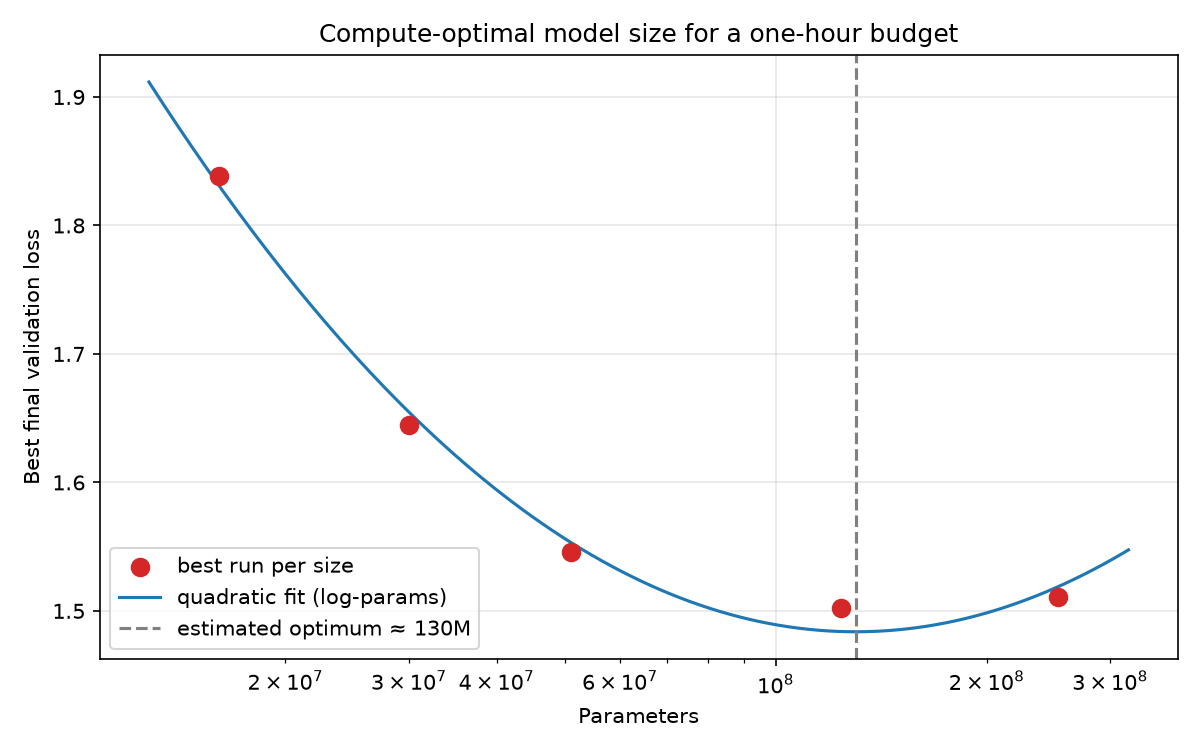
\includegraphics[width=0.49\linewidth]{figures/compute_optimal_fit.png}
  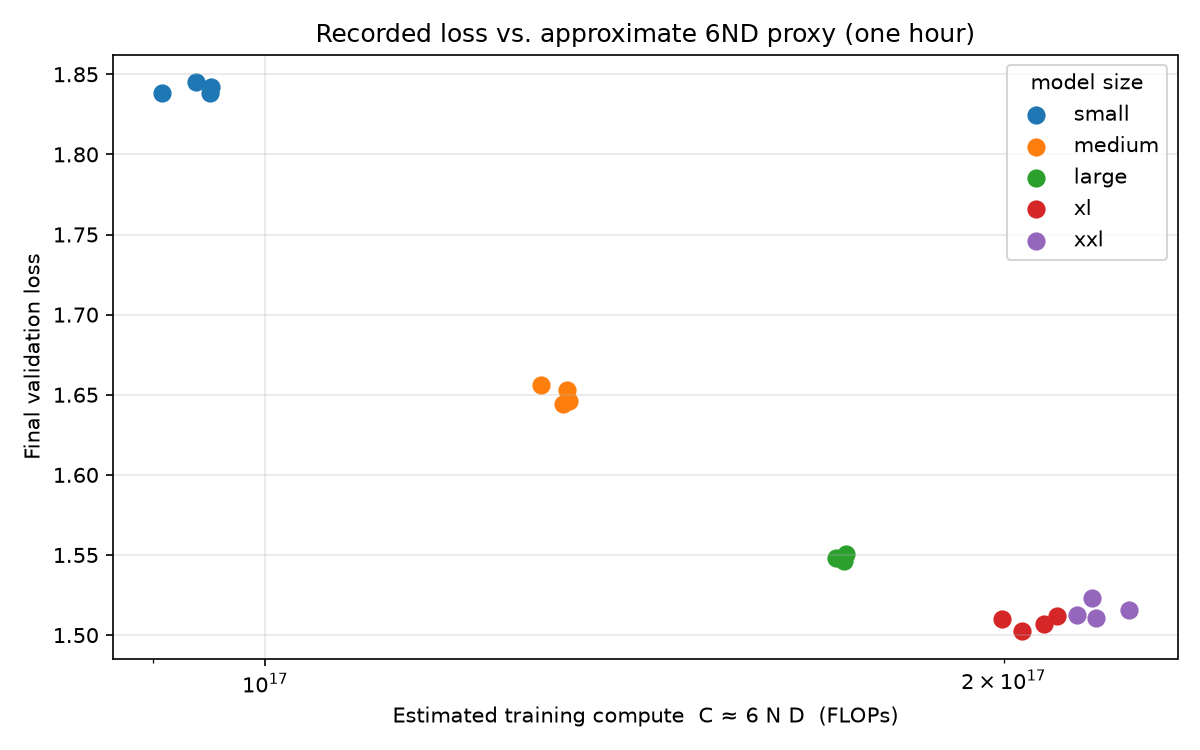
\includegraphics[width=0.49\linewidth]{figures/loss_vs_compute.png}
  \caption{Left: best validation loss per size against parameters, with a quadratic
  fit in log-parameters whose vertex estimates the compute-optimal size
  ($N^\star\approx130$M) for the one-hour budget, within noise of the empirical winner
  \texttt{xl}. Right: loss against estimated compute $C\approx6ND$; the smallest
  models deliver the least compute despite the identical wall-clock budget. The fit
  rests on five points, so read it as indicative, not precise.}
  \label{fig:optfit}
\end{figure}

\section{Discussion}
The winner wins because it sits where capacity and tokens balance for this budget: big
enough to hold what the smaller models cannot, small enough to still see enough tokens
in an hour to use that capacity. The whole experiment is compute-bound. Throughput,
not how much data is on hand, is the binding constraint, which is why the data
fraction hardly moves the loss and why \texttt{xxl} lands below \texttt{xl}. Give it a
bigger budget and we would expect the left panel of Fig.~\ref{fig:sizedata} to keep
bending to the right: \texttt{xxl} and larger should eventually pass \texttt{xl} once
they get enough tokens, and the data fraction should start to bite once a run can
actually finish a subset. A few caveats. Training samples windows with replacement, so
an hour guarantees neither a full epoch nor unique coverage. The single shared recipe
(learning rate, warmup, batch) is not tuned per size and may help some sizes more than
others. Validation used sampled windows rather than the full test-time pass. And the
TinyStories source revision is not pinned.

\section{Conclusion}
Under a fixed one-hour, from-scratch budget on one H100 MIG slice, the best language
model on TinyStories is \texttt{xl} at around 124M parameters; chosen on validation,
\texttt{xl\_data50} reaches test perplexity 4.41 (0.524 bits/byte). The trade-off that
matters most is throughput against capacity: because a bigger model gets through far
fewer tokens in the same wall-clock time, going bigger stops paying off, and then
backfires, well before the largest model we trained. How much training data a run is
allowed to touch makes almost no difference once you are this compute-bound.

\bibliographystyle{plainnat}
\bibliography{references}

\appendix
\section{Generated story samples}
The full set of samples for all 20 runs (five prompts each) lives in
\texttt{analysis/\allowbreak generations\_all.md}. As one example, both models continue
``\emph{Once upon a time}'' fluently, but the \texttt{xl} winner holds a longer, more
consistent story:

\paragraph{\texttt{small\_data25}.} \emph{``Once upon a time, there was a little girl
named Lily. Lily loved to play with her toys\ldots She painted a picture of a flower
and a house\ldots Later that day, Lily's mom asked her to help. Lily was happy to help
and started to decorate the room with pretty flowers.''} (The thread loops back on
itself.)

\paragraph{\texttt{xl\_data50} (selected).} \emph{``Once upon a time, there was a
little girl named Lily. Lily loved to play with her toys, especially her teddy bear.
One day, Lily's mommy asked her to help decorate the house for a party\ldots `Mommy,
can I carry my teddy bear?' she asked\ldots They arrived at the living room and Lily's
mommy gave her a big box of presents.''} (One plot, moving forward.)

\end{document}
